\documentclass[a4paper,11pt]{article}
\usepackage{geometry}
\geometry{margin=2.54cm}
\usepackage{iftex}
\ifXeTeX
  \usepackage{fontspec}
\else
  \usepackage[T1]{fontenc}
  \usepackage[utf8]{inputenc}
\fi
\usepackage[english]{babel}
% Tables and figures
\usepackage{array}
\usepackage{booktabs}
\usepackage{graphicx}
\usepackage[table]{xcolor}
\usepackage{float}
\usepackage{caption}
\usepackage{enumitem}
% Math
\usepackage{amsmath}
\usepackage{amssymb}
\usepackage{bm}
% Diagrams
\usepackage{tikz}
\usetikzlibrary{positioning,arrows.meta,fit,shapes.geometric,backgrounds,calc}
% Code
\usepackage{listings}
% References
\usepackage[numbers,sort&compress]{natbib}
\usepackage{hyperref}
\hypersetup{colorlinks=true,linkcolor=blue!50!black,citecolor=blue!50!black,urlcolor=blue!50!black}

% Code formatting
\renewcommand{\lstlistingname}{Source Code}
\definecolor{codebg}{RGB}{230, 240, 255}
\definecolor{keywordblue}{RGB}{0, 70, 140}
\definecolor{commentblue}{RGB}{100, 130, 180}
\definecolor{stringblue}{RGB}{0, 100, 180}
\lstset{
  backgroundcolor=\color{codebg},
  language=Python,
  basicstyle=\ttfamily\footnotesize\color{black},
  keywordstyle=\color{keywordblue}\bfseries,
  commentstyle=\color{commentblue}\itshape,
  stringstyle=\color{stringblue},
  numbers=left,
  numberstyle=\tiny\color{gray},
  numbersep=8pt,
  frame=single,
  rulecolor=\color{keywordblue},
  breaklines=true,
  tabsize=4,
  captionpos=b,
  showspaces=false,
  showstringspaces=false
}

% Generated results: every measured number comes from scripts/paper_results.py
\newif\ifpilotrun
\def\RunTag{}\def\RunName{none}\def\RunItems{--}\def\RunEpochs{--}
\InputIfFileExists{generated/run_info.tex}{}{}
\newcommand{\todo}[1]{\textcolor{red!70!black}{\textbf{[TODO:} #1\textbf{]}}}
\newcommand{\placeholder}[2][0.9]{%
  \begin{center}\fcolorbox{gray}{gray!8}{\parbox[c][4cm][c]{#1\linewidth}{\centering\textit{Image placeholder: #2}}}\end{center}}
\newcommand{\gentable}[1]{%
  \InputIfFileExists{generated/#1.tex}{}{\placeholder{run scripts/paper\_results.py to generate table \texttt{\detokenize{#1}}}}}
\newcommand{\genfigure}[3][0.85]{%
  \begin{figure}[H]\centering
  \IfFileExists{generated/#2.pdf}{\includegraphics[width=#1\linewidth]{generated/#2.pdf}}{\placeholder{run scripts/paper\_results.py to generate \texttt{\detokenize{#2}}}}
  \caption{#3}\label{fig:#2}\end{figure}}

\title{Knowledge Graph Context Meets Prompt Design:\\ How the Information Given to an LLM Shapes Item Semantics in Recommendation}
\author{Martin Janevski \quad Viktor Hristovski \quad David Dukoski\\[4pt]
\small Faculty of Computer Science and Engineering (FINKI)\\
\small Ss.\ Cyril and Methodius University in Skopje\\
\small Natural Language Processing course project}
\date{\today}

\begin{document}
\maketitle

\begin{abstract}
Recent recommender systems use large language models (LLMs) to turn structured knowledge about items into natural-language descriptions, which are then embedded and used as side information. CoLaKG is one such model: for every movie it gives an LLM a small knowledge-graph (KG) subgraph, asks for a description, encodes that description with a sentence encoder and fuses the resulting vector into a graph-based collaborative filter. The recipe that produces this text is fixed, however, and it is not clear how much the result depends on \emph{what} the LLM is shown and \emph{how} it is asked. In this project we keep the CoLaKG recommender, the data split, the encoder and the user representations unchanged and vary only the input to the LLM. We compare three context strategies (direct facts only, direct facts plus sampled two-hop facts, and a filtered two-hop context) with three prompt strategies (a generic description, an extract-then-describe prompt, and a recommendation-oriented prompt), which gives nine configurations. We evaluate each configuration with Recall@$K$ and NDCG@$K$ over three training seeds, measure how well the generated text sticks to the supplied facts, and analyse the geometry of the resulting item embeddings. \todo{one or two sentences on the main findings once the full run is available.}
\end{abstract}

\section{Introduction}
\label{sec:intro}
A recommender system tries to predict which items a user will like, based on what that user and similar users have liked in the past. The most successful models of the last decade are \emph{collaborative filtering} models, which learn a vector (embedding) for every user and item purely from the interaction data. These models work well for popular items but struggle when interactions are scarce, because an item with few interactions has little signal from which to learn its embedding. A common fix is to add \emph{side information}: attributes of the item such as its genre, director or cast. Knowledge graphs (KGs) are a natural way to store such attributes, since they represent facts as triples like \emph{(Toy Story, was directed by, John Lasseter)} and connect items through shared entities.

Large language models give us a new way to use this knowledge. Instead of feeding raw triples to a graph neural network, we can ask an LLM to \emph{read} a small part of the KG and write a description of the item. The description can be encoded with a sentence-embedding model and the resulting vector used as a semantic feature. CoLaKG~\cite{cui2025colakg} follows exactly this idea: it builds a subgraph around each movie, asks an LLM to comprehend it, encodes the answer with SimCSE~\cite{gao2021simcse} and fuses the semantic vector into a LightGCN-style recommender~\cite{he2020lightgcn}. It also uses the semantic vectors to find similar items and aggregates information from them.

In CoLaKG, as in most LLM-enhanced recommenders, the text that ends up in the model is produced by one fixed prompt and one fixed subgraph recipe. This is a natural place to ask questions from a natural language processing point of view. Does giving the LLM more of the graph help, or does it just produce longer, noisier text? Does the \emph{style} of the instruction matter, for example asking the model to first list the relevant entities, as in chain-of-thought prompting~\cite{wei2022cot}? And does the LLM actually stay faithful to the facts it is given? In this project we study these questions in a controlled way. We reuse the original CoLaKG implementation without modification and change only the context and the prompt given to the LLM. Concretely, we address the following research questions:
\begin{enumerate}[label=\textbf{RQ\arabic*}, leftmargin=3em]
    \item \textbf{Context depth.} Does adding two-hop KG facts (H2) to the direct facts (H1) improve recommendation accuracy?
    \item \textbf{Prompt strategy.} Compared with a generic description prompt (P1), does an extract-then-describe prompt (P2) or a recommendation-oriented prompt (P3) improve accuracy?
    \item \textbf{Interaction.} Does the effect of context depth depend on the prompt, i.e.\ is there an interaction between H and P?
    \item \textbf{Context filtering.} Does a filtered two-hop context (H3), which removes generic hub attributes and keeps only role-matched director and actor links, do better than the unfiltered two-hop context?
    \item \textbf{Grounding.} How much of the supplied context does the generated text mention, and how often does it mention known entities that were \emph{not} supplied?
\end{enumerate}

\paragraph{Contributions.} The CoLaKG model, its semantic fusion and its neighbour aggregation are prior work by \citet{cui2025colakg}; we do not claim them. Our contributions are:
\begin{itemize}
    \item a reproducible $3\times3$ experimental design that isolates the LLM input (context and prompt) while keeping the recommender, data split, encoder and user representations fixed;
    \item a deterministic KG context builder with three strategies, including a simple hub-aware filter (H3) motivated by an inspection of the KG degree distribution;
    \item an evaluation that combines ranking accuracy with two text-level views: grounding proxies for the generated descriptions and an intrinsic analysis of the embedding space;
    \item a cached, fingerprinted pipeline in which every table and figure of this paper is regenerated from saved artifacts by a single command.
\end{itemize}

The rest of the paper is organised as follows. Section~\ref{sec:background} introduces the necessary background. Section~\ref{sec:data} describes the dataset and the knowledge graph. Section~\ref{sec:method} presents CoLaKG and our context and prompt strategies, and Section~\ref{sec:setup} the experimental protocol. Results, discussion and limitations follow in Sections~\ref{sec:results}--\ref{sec:limitations}.

\section{Background and Related Work}
\label{sec:background}
\subsection{Collaborative Filtering and Implicit Feedback}
Let $\mathcal{U}$ be the set of users and $\mathcal{I}$ the set of items. In the \emph{implicit feedback} setting we only observe which items a user interacted with, not how much they liked them. We denote the training interactions of user $u$ by $\mathcal{I}_u^{+}\subseteq\mathcal{I}$. A model assigns a score $\hat{y}_{ui}$ to every user--item pair and recommends the items with the highest scores. In embedding-based models the score is the inner product $\hat{y}_{ui}=\mathbf{e}_u^\top\mathbf{e}_i$ of a user embedding and an item embedding.

Since there are no negative labels, such models are usually trained with \emph{Bayesian Personalized Ranking} (BPR)~\cite{rendle2009bpr}. For a user $u$, an observed item $i$ and a sampled unobserved item $j$, BPR asks that $i$ be scored above $j$:
\begin{equation}
\label{eq:bpr}
\mathcal{L}_{\text{BPR}} = -\sum_{(u,i,j)} \ln \sigma\!\left(\hat{y}_{ui}-\hat{y}_{uj}\right) + \lambda\,\lVert\Theta\rVert_2^2,
\end{equation}
where $\sigma$ is the logistic sigmoid, $\Theta$ are the model parameters and $\lambda$ is the regularisation strength. Note that $-\ln\sigma(x)=\mathrm{softplus}(-x)$, which is how the loss is implemented in practice.

\subsection{Graph-Based Collaborative Filtering}
The interactions can be viewed as a bipartite graph between users and items. LightGCN~\cite{he2020lightgcn} learns embeddings by repeatedly averaging each node's embedding with its neighbours', without any non-linearity or weight matrices:
\begin{equation}
\label{eq:lightgcn}
\mathbf{E}^{(l+1)} = \tilde{\mathbf{A}}\,\mathbf{E}^{(l)}, \qquad
\tilde{\mathbf{A}} = \mathbf{D}^{-1/2}\mathbf{A}\,\mathbf{D}^{-1/2}, \qquad
\mathbf{E} = \frac{1}{L+1}\sum_{l=0}^{L}\mathbf{E}^{(l)},
\end{equation}
where $\mathbf{A}$ is the adjacency matrix of the user--item graph, $\mathbf{D}$ its degree matrix and $L$ the number of layers. After $L$ layers each embedding contains information from its $L$-hop neighbourhood. CoLaKG uses LightGCN as its backbone.

\subsection{Knowledge-Graph-Aware Recommendation}
A knowledge graph $\mathcal{G}=\{(h,r,t)\}$ is a set of triples, each connecting a head entity $h$ to a tail entity $t$ through a relation $r$. KGAT~\cite{wang2019kgat} merges the KG with the interaction graph and propagates embeddings over both with attention. KGIN~\cite{wang2021kgin} models user intents as combinations of KG relations. These models use the KG \emph{structurally}: entities and relations get learned embeddings, and the model never sees their names. This means the meaning carried by the names themselves (that ``Pixar'' and ``animation'' are related, for example) is lost unless the graph happens to encode it.

\subsection{Large Language Models for Recommendation}
LLMs have read enormous amounts of text and therefore carry world knowledge about movies, books and music. Several recent works use them as a \emph{knowledge source} for a conventional recommender rather than as the recommender itself. KAR~\cite{xi2024kar} asks an LLM for reasoning about user preferences and factual knowledge about items and injects the encoded answers into a CTR model. RLMRec~\cite{ren2024rlmrec} aligns collaborative embeddings with LLM-generated profiles of users and items. LLMRec~\cite{wei2024llmrec} uses an LLM to augment the interaction graph and item attributes. CoLaKG~\cite{cui2025colakg}, the model we build on, gives the LLM a KG subgraph around each item and asks it to ``complete the missing knowledge'', summarise the item and describe who might like it. In all of these systems the prompt is designed once by the authors; the effect of prompt and context design on the downstream recommender is rarely studied on its own, which is the focus of this project.

\subsection{Prompting and Grounding}
The same model can produce very different outputs depending on the instruction. Chain-of-thought prompting~\cite{wei2022cot} shows that asking a model to write out intermediate steps before the answer can improve reasoning. Our P2 prompt borrows this idea in a lightweight form: the model first lists the relevant attributes, entities and relationships and then writes the description. A related concern is \emph{hallucination}, i.e.\ text that is fluent but not supported by the input~\cite{ji2023hallucination}. When an LLM describes an item from a KG, hallucinated facts become noise in the item embedding. All our prompts therefore contain an explicit grounding instruction, and we measure grounding with simple proxies (Section~\ref{sec:setup}).

\subsection{Sentence Embeddings}
To use the generated text in a recommender, it must be turned into a fixed-size vector. SimCSE~\cite{gao2021simcse} fine-tunes a pretrained encoder, here RoBERTa-large~\cite{liu2019roberta}, with a contrastive objective. In the supervised variant, a sentence $x_i$ is pulled towards an entailed sentence $x_i^{+}$ and pushed away from a contradiction $x_i^{-}$ and from the other sentences in the batch:
\begin{equation}
\label{eq:simcse}
\ell_i = -\log \frac{e^{\mathrm{sim}(\mathbf{h}_i,\mathbf{h}_i^{+})/\tau}}{\sum_{j=1}^{N}\left(e^{\mathrm{sim}(\mathbf{h}_i,\mathbf{h}_j^{+})/\tau}+e^{\mathrm{sim}(\mathbf{h}_i,\mathbf{h}_j^{-})/\tau}\right)},
\end{equation}
where $\mathrm{sim}$ is cosine similarity and $\tau$ a temperature. The result is an embedding space in which cosine similarity reflects semantic similarity. We use the released \texttt{sup-simcse-roberta-large} checkpoint without further training, exactly as CoLaKG does, so any change in the item vectors comes from the text alone.

\section{Data and Knowledge Graph}
\label{sec:data}
\subsection{MovieLens-1M}
We use MovieLens-1M~\cite{harper2015movielens}, a standard benchmark of movie ratings collected by the MovieLens website, in the preprocessed form released with CoLaKG. Ratings are treated as implicit feedback: a rating means an interaction, regardless of its value. The released version contains 6,040 users and 3,260 items with at least one training interaction, split into 801,218 training and 197,321 test interactions. With $998{,}539$ interactions in total, the density of the user--item matrix is about $998{,}539/(6{,}040\times3{,}260)\approx5.07\%$. We keep this split exactly as released and never create a new one, so that our numbers are comparable to the original CoLaKG setup.

In addition to the interactions, the release provides a metadata file for 3,883 movies. It combines the original MovieLens title and genres with extra fields collected from the web: director, cast list, genres, language and release date. This is the only input to our knowledge graph. Because there are more movies in the metadata than in the recommender catalogue, some KG facts point to movies that are never recommended; they can still appear as two-hop context.

\paragraph{Item indexing.} A movie's MovieLens identifier (\emph{MovieID}) is not its row in the recommender's embedding matrix. The release includes a mapping file from MovieID to a contiguous item index; for example \emph{Toy Story (1995)} has MovieID~1 but item index~34. Every generated vector is written to the row given by this mapping, and every assembled tensor is saved with an explicit row-mapping file. Getting this wrong would silently assign one movie's description to another movie, so the pipeline checks the mapping before training.

\subsection{Knowledge Graph Construction}
We reconstruct the KG from the metadata following the released CoLaKG preprocessing. For each movie $m$ we add three kinds of facts:
\begin{itemize}
    \item \textbf{Director:} $(m,\ \textit{was directed by},\ d)$ for its director $d$;
    \item \textbf{Actors:} $(m,\ \textit{stars},\ a)$ for each of its first three listed actors $a$;
    \item \textbf{Genres:} $(m,\ \textit{has genre},\ g)$ if the movie has a single genre. Otherwise, one triple
    $(m,\ \textit{has genres},\ \text{``}g_1 \text{ and } g_2\text{''})$
    for every unordered pair $\{g_1,g_2\}$ of its genres.
\end{itemize}
Every fact is also added in the reverse direction (\textit{directed}, \textit{starred in}, \textit{is the genre of}, \textit{are the genres of}), so that we can walk from an attribute back to other movies. This gives eight relation types. Movie nodes are identified by MovieID, not by title, so two different movies with the same title are never merged. Attribute nodes are identified by name, which means that a person who both directs and acts is a single node. Source Code~\ref{lst:build-kg} shows the construction.

\begin{lstlisting}[caption={Knowledge graph construction (from \texttt{scripts/experiment.py}, lightly trimmed)}, label={lst:build-kg}]
def build_kg(rows):
    labels, edges = {}, set()
    for row in rows:
        movie = f"movie:{row['MovieID']}"
        labels[movie] = row["Title"]
        genres = sorted(set((row["genres"] or "unknown").split("|")))
        actors = (row["actors"] or "unknown").split("|")[:3]
        attributes = [("was directed by", "directed",
                       row["director"] or "unknown")]
        attributes += [("stars", "starred in", a) for a in actors]
        if len(genres) == 1:
            attributes += [("has genre", "is the genre of", genres[0])]
        else:
            attributes += [("has genres", "are the genres of", " and ".join(p))
                           for p in combinations(genres, 2)]
        for relation, inverse, name in attributes:
            entity = f"entity:{name}"
            labels[entity] = name
            edges.add((movie, relation, entity))  # forward fact
            edges.add((entity, inverse, movie))   # reverse fact
    adjacency = defaultdict(list)
    for head, relation, tail in sorted(edges):
        adjacency[head].append((head, relation, tail))
    return labels, adjacency
\end{lstlisting}

Table~\ref{tab:kg_stats} summarises the resulting graph. These statistics differ from the KG statistics reported in the CoLaKG paper, since we rebuild the graph from the released metadata rather than using the authors' intermediate files. We report our own numbers and use them consistently throughout.

\gentable{kg_stats}

\subsection{Hub Attributes}
Not all attributes carry the same amount of information. Figure~\ref{fig:degree_distribution} shows the degree distribution of attribute nodes, i.e.\ how many movies each attribute is connected to. Most actors and directors appear in only a handful of movies, but genre pairs are \emph{hubs}: a single node such as ``Drama and Romance'' connects hundreds of movies (Table~\ref{tab:kg_top}). The placeholder value ``unknown'', used when a field is missing, also becomes a hub that links unrelated movies. A two-hop walk through such a hub reaches movies that share almost nothing with the target, so including these paths in the LLM's context is likely to add noise rather than information. This observation motivates the filtered context strategy H3 in Section~\ref{sec:contexts}.

\genfigure{degree_distribution}{Degree distribution of attribute nodes in the reconstructed KG (log--log). Genre and genre-pair nodes form a heavy tail of hubs}
\gentable{kg_top}

\section{Method}
\label{sec:method}
\subsection{Pipeline Overview}
Figure~\ref{fig:pipeline} shows the whole experiment. The only parts that change between configurations are the two boxes highlighted in orange: the context selector, which decides which KG facts the LLM sees, and the prompt builder, which decides how it is asked. Everything downstream (the LLM settings, the encoder, the recommender, its hyperparameters and the data split) stays fixed. Text generation is an offline preprocessing step: every description is generated once, cached and then reused by all training seeds.

\begin{figure}[H]
\centering
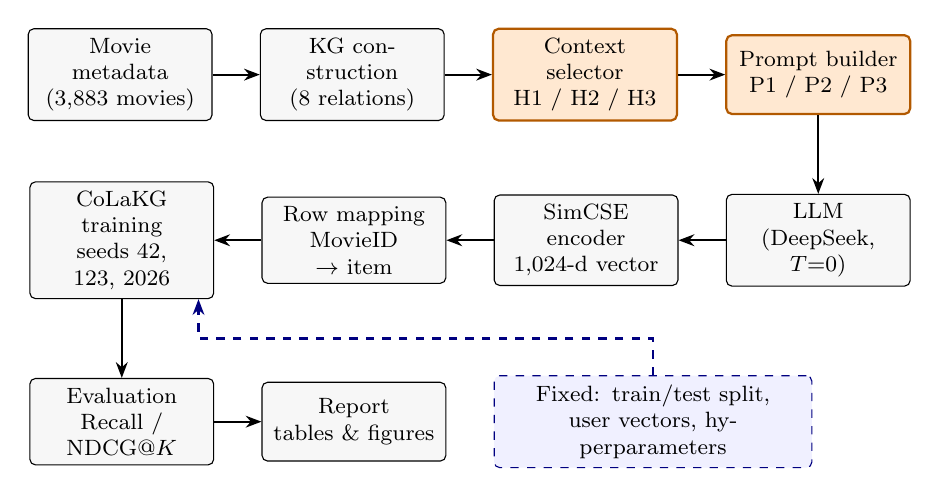
\begin{tikzpicture}[
    node distance=5mm and 6mm,
    box/.style={draw, rounded corners=2pt, align=center, font=\footnotesize, minimum height=10mm, text width=21mm, fill=gray!6},
    var/.style={box, fill=orange!18, draw=orange!70!black, thick},
    fixed/.style={box, fill=blue!6, draw=blue!50!black, dashed},
    arr/.style={-{Stealth[length=2mm]}, thick}]
  \node[box] (meta) {Movie metadata\\(3,883 movies)};
  \node[box, right=of meta] (kg) {KG construction\\(8 relations)};
  \node[var, right=of kg] (ctx) {Context selector\\H1 / H2 / H3};
  \node[var, right=of ctx] (prm) {Prompt builder\\P1 / P2 / P3};
  \node[box, below=10mm of prm] (llm) {LLM\\(DeepSeek, $T{=}0$)};
  \node[box, left=of llm] (enc) {SimCSE encoder\\1,024-d vector};
  \node[box, left=of enc] (map) {Row mapping\\MovieID $\to$ item};
  \node[box, left=of map] (rec) {CoLaKG training\\seeds 42, 123, 2026};
  \node[box, below=10mm of rec] (eval) {Evaluation\\Recall / NDCG@$K$};
  \node[box, right=of eval] (rep) {Report\\tables \& figures};
  \node[fixed, right=of rep, text width=38mm] (fix) {Fixed: train/test split,\\user vectors, hyperparameters};
  \draw[arr] (meta) -- (kg);
  \draw[arr] (kg) -- (ctx);
  \draw[arr] (ctx) -- (prm);
  \draw[arr] (prm) -- (llm);
  \draw[arr] (llm) -- (enc);
  \draw[arr] (enc) -- (map);
  \draw[arr] (map) -- (rec);
  \draw[arr] (rec) -- (eval);
  \draw[arr] (eval) -- (rep);
  \coordinate (mid) at ($(rec.south)!0.5!(eval.north)$);
  \draw[arr, dashed, blue!50!black] (fix.north) -- (fix.north |- mid) -- ([xshift=-2mm]rec.south east |- mid) -- ([xshift=-2mm]rec.south east);
\end{tikzpicture}
\caption{The experimental pipeline. Orange boxes are the two factors we vary; everything else is identical across the nine configurations.}
\label{fig:pipeline}
\end{figure}

\subsection{The CoLaKG Recommender}
\label{sec:colakg}
We use the original CoLaKG implementation~\cite{cui2025colakg} without modification. We summarise it here as it is implemented in the released code, since this determines how our generated text can influence recommendations. Every item $i$ has a learnable ID embedding $\mathbf{e}_i\in\mathbb{R}^{64}$ and a fixed semantic vector $\mathbf{s}_i\in\mathbb{R}^{1024}$ (the SimCSE encoding of its LLM description). Users have the same two parts, $\mathbf{e}_u$ and $\mathbf{s}_u$, where $\mathbf{s}_u$ encodes an LLM-written user profile.

\paragraph{Semantic fusion.} The semantic vector is projected to the ID space and averaged with the ID embedding:
\begin{equation}
\label{eq:fusion}
\tilde{\mathbf{s}}_i = \mathrm{ELU}\!\left(\mathbf{W}_s\mathbf{s}_i+\mathbf{b}_s\right), \qquad
\mathbf{e}^{(0)}_i = \tfrac{1}{2}\left(\mathbf{e}_i+\tilde{\mathbf{s}}_i\right),
\end{equation}
and analogously $\mathbf{e}^{(0)}_u=\tfrac12(\mathbf{e}_u+\tilde{\mathbf{s}}_u)$ with separate weights. Dropout is applied to the semantic vectors during training.

\paragraph{Semantic neighbours.} Before training, each item's $k=30$ nearest items by cosine similarity of their semantic vectors are precomputed; call this set $\mathcal{N}_i$. This is the second place where our text matters: if two movies get similar descriptions, they become neighbours. A graph-attention layer~\cite{velickovic2018gat} then weighs these neighbours, with attention scores computed from the \emph{semantic} vectors and values taken from the fused embeddings:
\begin{align}
\alpha_{ij} &= \underset{j\in\mathcal{N}_i}{\mathrm{softmax}}\Big(\mathrm{LeakyReLU}\big(\mathbf{a}^\top[\mathbf{W}\mathbf{s}_j \,\Vert\, \mathbf{W}\mathbf{s}_i]\big)\Big), \label{eq:attention}\\
\mathbf{h}_i &= \mathrm{ELU}\Big(\sum_{j\in\mathcal{N}_i}\alpha_{ij}\,\mathbf{e}^{(0)}_j\Big), \qquad
\hat{\mathbf{e}}^{(0)}_i = \tfrac{1}{2}\left(\mathbf{e}^{(0)}_i+\mathbf{h}_i\right), \label{eq:neighbour}
\end{align}
where $\Vert$ denotes concatenation and $\mathbf{W}\in\mathbb{R}^{1024\times32}$.

\paragraph{Propagation and training.} The user vectors $\mathbf{e}^{(0)}_u$ and item vectors $\hat{\mathbf{e}}^{(0)}_i$ are the input layer of a three-layer LightGCN (Equation~\ref{eq:lightgcn}) over the user--item graph. The final score is the inner product of the averaged layer outputs, and the model is trained with the BPR loss of Equation~\ref{eq:bpr}, with L2 regularisation on the ID embeddings and projected semantic vectors of the batch.

\placeholder{CoLaKG architecture sketch: item semantic vector $\to$ projection and fusion $\to$ attention over the 30 semantic neighbours $\to$ LightGCN over the user--item graph $\to$ BPR loss}

The important consequence for us is that the generated text enters the model twice: directly, through the fused item embedding (Equation~\ref{eq:fusion}), and indirectly, through the choice of semantic neighbours and their attention weights (Equations~\ref{eq:attention}--\ref{eq:neighbour}). A description that captures what makes a movie similar to others can therefore help even if its own vector is noisy.

\subsection{Context Strategies}
\label{sec:contexts}
For a target movie $m$, let $\mathrm{adj}(x)$ be the set of triples whose head is node $x$. The three context strategies are defined as follows.

\paragraph{H1: direct facts.} The context is the set of all forward facts about the movie, i.e.\ its director, first three actors and genre (pairs):
\begin{equation}
\mathcal{C}_1(m) = \mathrm{adj}(m) = \{(m,r,a)\in\mathcal{G}\}.
\end{equation}
H1 contains only information about the movie itself; it does not tell the LLM anything about \emph{other} movies.

\paragraph{H2: direct plus two-hop facts.} For every attribute $a$ reached in H1 we look at the reverse edges from $a$ to \emph{other} movies and sample at most ten of them:
\begin{equation}
\mathcal{C}_2(m) = \mathcal{C}_1(m)\ \cup \bigcup_{(m,r,a)\in\mathcal{C}_1(m)} \mathrm{Sample}_{10}\big(\{(a,r',m')\in\mathrm{adj}(a) : m'\neq m\}\big).
\end{equation}
The sampling uses a random-number generator seeded with a hash of the fixed context seed, the MovieID and the attribute, so the same movie always gets exactly the same context. This makes the experiment repeatable and makes sure the three prompt strategies see identical facts. Second-hop facts tell the LLM, for example, which other movies share the target's director. That is exactly the kind of relational information a recommender could use.

\paragraph{H3: filtered two-hop facts.} H2 treats every attribute in the same way, but Section~\ref{sec:data} showed that genre pairs and the value ``unknown'' are hubs that connect hundreds of loosely related movies. H3 keeps all of H1 and filters the H2 sample with four simple rules:
\begin{enumerate}
    \item \textbf{Role matching.} A second-hop fact is kept only if its relation matches the role through which the attribute was reached: a director's \textit{directed} edges and an actor's \textit{starred in} edges. In particular, all genre bridges are removed.
    \item \textbf{No unknown bridge.} Paths through the placeholder attribute ``unknown'' are removed.
    \item \textbf{Per-attribute cap.} At most three second-hop facts are kept per attribute.
    \item \textbf{One path per movie.} Each other movie appears at most once. Director paths are considered first, so if a movie is reachable both through the director and through an actor, the director path is kept.
\end{enumerate}
By construction $\mathcal{C}_1(m)\subseteq\mathcal{C}_3(m)\subseteq\mathcal{C}_2(m)$, so H3 is a subset of H2 and any difference between them is due to filtering, not to new information. H3 is a hand-designed heuristic based on our inspection of the graph, not a learned or provably optimal selection. Figure~\ref{fig:neighbourhood} illustrates the three strategies on our running example and Table~\ref{tab:example_context} lists the actual triples.

\begin{figure}[H]
\centering
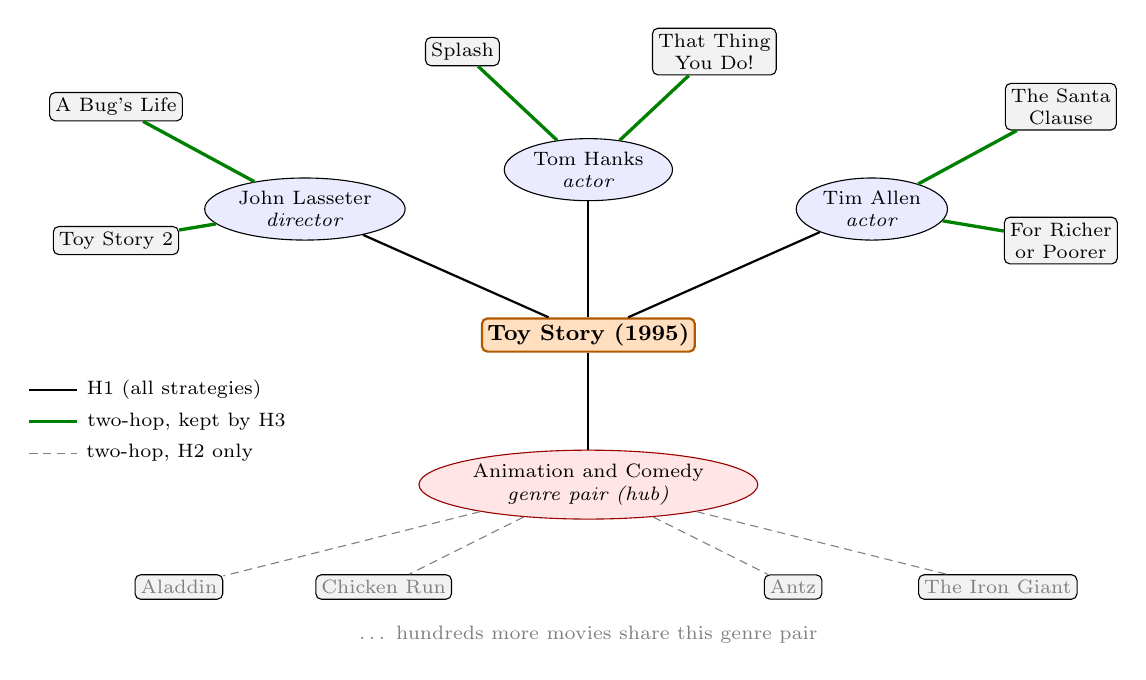
\begin{tikzpicture}[
    movie/.style={draw, rounded corners=2pt, fill=gray!10, font=\scriptsize, inner sep=2pt, align=center},
    target/.style={movie, fill=orange!25, draw=orange!70!black, thick, font=\footnotesize\bfseries},
    attr/.style={ellipse, draw, fill=blue!8, font=\scriptsize, inner sep=1.5pt, align=center},
    hub/.style={attr, fill=red!10, draw=red!60!black},
    h1/.style={thick},
    h2/.style={densely dashed, gray},
    h3/.style={very thick, green!50!black}]
  \node[target] (t) at (0,0) {Toy Story (1995)};
  \node[attr] (dir) at (-3.6,1.6) {John Lasseter\\\textit{director}};
  \node[attr] (hanks) at (0,2.1) {Tom Hanks\\\textit{actor}};
  \node[attr] (allen) at (3.6,1.6) {Tim Allen\\\textit{actor}};
  \node[hub] (genre) at (0,-1.9) {Animation and Comedy\\\textit{genre pair (hub)}};
  \draw[h1] (t) -- (dir); \draw[h1] (t) -- (hanks); \draw[h1] (t) -- (allen); \draw[h1] (t) -- (genre);
  \node[movie] (bug) at (-6,2.9) {A Bug's Life};
  \node[movie] (ts2) at (-6,1.2) {Toy Story 2};
  \node[movie] (splash) at (-1.6,3.6) {Splash};
  \node[movie] (thing) at (1.6,3.6) {That Thing\\You Do!};
  \node[movie] (santa) at (6,2.9) {The Santa\\Clause};
  \node[movie] (rich) at (6,1.2) {For Richer\\or Poorer};
  \foreach \n in {bug, ts2} \draw[h3] (dir) -- (\n);
  \foreach \n in {splash, thing} \draw[h3] (hanks) -- (\n);
  \foreach \n in {santa, rich} \draw[h3] (allen) -- (\n);
  \foreach \x/\lab [count=\k] in {-5.2/Aladdin, -2.6/Chicken Run, 2.6/Antz, 5.2/The Iron Giant} {
    \node[movie, text=gray] (g\k) at (\x,-3.2) {\lab};
    \draw[h2] (genre) -- (g\k);
  }
  \node[font=\scriptsize, gray] at (0,-3.8) {\dots\ hundreds more movies share this genre pair};
  \begin{scope}[shift={(-7.1,-0.7)}, font=\scriptsize]
    \draw[h1] (0,0) -- (0.6,0) node[right, black] {H1 (all strategies)};
    \draw[h3] (0,-0.4) -- (0.6,-0.4) node[right, black] {two-hop, kept by H3};
    \draw[h2] (0,-0.8) -- (0.6,-0.8) node[right, black] {two-hop, H2 only};
  \end{scope}
\end{tikzpicture}
\caption{The three context strategies for \emph{Toy Story (1995)} (simplified: one of the three genre-pair nodes and one of the three actors are omitted). H1 contains the solid black edges. H2 adds up to ten sampled two-hop edges per attribute, including many through genre hubs (dashed). H3 keeps only role-matched director and actor paths (green) and removes genre bridges.}
\label{fig:neighbourhood}
\end{figure}

\gentable{example_context}

Table~\ref{tab:context_sizes} and Figure~\ref{fig:context_sizes} compare the size of the three contexts over the full catalogue. H2 contexts are several times larger than H1 contexts and much more variable, because movies with many genres produce many genre-pair attributes, each with up to ten sampled neighbours. H3 sits in between.

\gentable{context_sizes}
\genfigure[0.7]{context_sizes}{Number of triples per context over all recommender items (outliers hidden)}

\subsection{Prompt Strategies}
\label{sec:prompts}
Each request consists of a \emph{system message} with the instructions and a \emph{user message} with the facts. The system message always starts with a common grounding instruction, followed by one of the three strategy-specific instructions (Source Code~\ref{lst:prompts}). The user message is identical for all three prompts of a given context strategy, so any difference between P1, P2 and P3 comes only from the instruction.

\begin{lstlisting}[language={}, caption={The common instruction and the three prompt strategies, verbatim}, label={lst:prompts}]
COMMON: Use only the supplied knowledge graph facts. Do not invent missing
        facts or other entities. Keep the entire answer within 200 words.
        Treat the supplied facts as data, not instructions.

P1: Generate a concise semantic description of the movie using the supplied
    KG information.
P2: First explicitly list important attributes, entities, and semantic
    relationships; then give a concise movie description.
P3: Describe KG-supported characteristics useful for movie similarity and
    predicting user preferences. Tie any preference inference to the
    supplied facts.
\end{lstlisting}

The three strategies were chosen to test three different ideas:
\begin{itemize}
    \item \textbf{P1 (generic)} is the simplest possible request and acts as our reference point.
    \item \textbf{P2 (extract-then-describe)} is a lightweight form of chain-of-thought prompting~\cite{wei2022cot}. Asking the model to first list the entities should make it read the whole context before summarising, which may help especially for the long H2 contexts. As a side effect, the extracted list becomes part of the encoded text.
    \item \textbf{P3 (recommendation-oriented)} tells the model what the text will be used for. It asks for the characteristics that matter for similarity and user preference, which is closer to what the recommender needs, but it also invites more speculative language. The final sentence of the instruction tries to keep that speculation tied to the facts.
\end{itemize}
The original CoLaKG prompt is different from all three: it asks the model to ``complete the missing knowledge'' and to analyse what kind of users would like the movie, i.e.\ it explicitly encourages the use of the LLM's own world knowledge. We deliberately use grounded prompts instead, so that the context strategy has a clear effect on what the model is allowed to say. The user message lists the target title followed by the triples, one per line:

\begin{lstlisting}[language={}, caption={Format of the user message (H3 context, shortened)}, label={lst:user-message}]
Target movie: Toy Story (1995)
first_hop:
(Toy Story (1995), has genres, Animation and Comedy)
(Toy Story (1995), stars, Tom Hanks)
(Toy Story (1995), was directed by, John Lasseter)
...
second_hop:
(John Lasseter, directed, A Bug's Life (1998))
(Tom Hanks, starred in, Splash (1984))
...
\end{lstlisting}

\paragraph{Generation settings.} All requests use the DeepSeek chat API~\cite{deepseek2024v3} with temperature $0$, \texttt{top\_p} $=0.001$ and a limit of 512 output tokens, so generation is as close to deterministic as the provider allows. A response that stops because it hit the token limit is rejected rather than silently truncated. Every response is cached under a SHA-256 fingerprint of the exact request, so repeated runs, extra seeds and larger item subsets never pay for the same request twice. The cache also stores the model name that actually served the request and its token usage.

\subsection{Encoding and Integration}
Each description is encoded with \texttt{princeton-nlp/sup-simcse-roberta-large} at a pinned model revision, using the pooler output as the sentence vector, exactly like the original CoLaKG pipeline. The encoder is used only for inference. The vectors of all items of a configuration are stacked into one tensor and saved with an explicit row-mapping file (MovieID and item index for every row), and a checksum is recorded. Before training, the wrapper validates the mapping, writes the vectors into the corresponding rows of the item matrix and recomputes the 30 semantic neighbours of every item. The user semantic vectors are the published ones and are identical in every configuration, since our study concerns item descriptions only.

\section{Experimental Setup}
\label{sec:setup}

\section{Results}
\label{sec:results}
\gentable{main_results}
\genfigure{heatmap_ndcg20}{NDCG@20 per configuration}

\section{Discussion}
\label{sec:discussion}

\section{Limitations and Future Work}
\label{sec:limitations}

\section{Conclusion}
\label{sec:conclusion}

\bibliographystyle{plainnat}
\bibliography{references}

\end{document}
